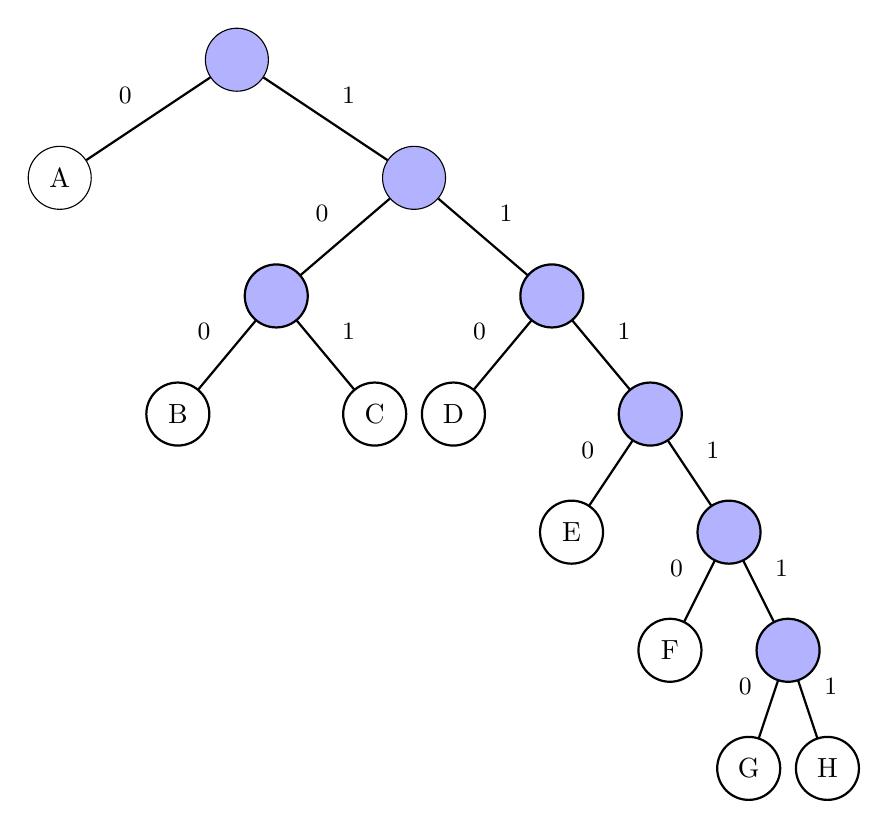
\begin{tikzpicture}[
    level distance=1.5cm,
    level 1/.style={sibling distance=4.5cm},
    level 2/.style={sibling distance=3.5cm},
    level 3/.style={sibling distance=2.5cm},
    level 4/.style={sibling distance=2cm},
    level 5/.style={sibling distance=1.5cm},
    level 6/.style={sibling distance=1cm},
    every node/.style={circle, fill=blue!30, draw, minimum size=8mm},
    leaf/.style={circle, fill=white, draw, minimum size=8mm, font=\normalsize},
    edge from parent/.style={draw, thick},
    edge label/.style={font=\small, fill=none, draw=none} % Rimosso 'auto'
]

\node {}
    child {
        node[leaf] {A}
        edge from parent node[above left, edge label] {0} % Modificato qui
    }
    child {
        node {} % Nodo P1
        child {
            node {} % Nodo P_BC, genitore diretto di B e C
            child {
                node[leaf] {B}
                edge from parent node[above left, edge label] {0} % Modificato qui
            }
            child {
                node[leaf] {C}
                edge from parent node[above right, edge label] {1} % Modificato qui
            }
            edge from parent node[above left, edge label] {0} % Modificato qui (arco da P1 a P_BC)
        }
        child {
            node {} % Nodo P_D, genitore di D
            child {
                node[leaf] {D}
                edge from parent node[above left, edge label] {0} % Modificato qui
            }
            child {
                node {} % Genitore di E
                child {
                    node[leaf] {E}
                    edge from parent node[above left, edge label] {0} % Modificato qui
                }
                child {
                    node {} % Genitore di F
                    child {
                        node[leaf] {F}
                        edge from parent node[above left, edge label] {0} % Modificato qui
                    }
                    child {
                        node {} % Genitore di G e H
                        child {
                            node[leaf] {G}
                            edge from parent node[above left, edge label] {0} % Modificato qui
                        }
                        child {
                            node[leaf] {H}
                            edge from parent node[above right, edge label] {1} % Modificato qui
                        }
                        edge from parent node[above right, edge label] {1} % Modificato qui
                    }
                    edge from parent node[above right, edge label] {1} % Modificato qui
                }
                edge from parent node[above right, edge label] {1} % Modificato qui
            }
            edge from parent node[above right, edge label] {1} % Modificato qui (arco da P1 a P_D)
        }
        edge from parent node[above right, edge label] {1} % Modificato qui (arco dalla Radice a P1)
    };

\end{tikzpicture}